% written by scripts/reuse_short.py from the sources of the short paper; do not edit
Five arms share one model server, one withheld agent bundle, google-adk 1.36.1 and all sampling settings.

\begin{table}[!tb]
\centering
\caption{Arms; changes in percentage points.}\label{tab:casearms}
\footnotesize
\begin{tabular}{@{}
  >{\raggedright\arraybackslash}p{(\linewidth - 6\tabcolsep) * \real{0.0500}}
  >{\raggedright\arraybackslash}p{(\linewidth - 6\tabcolsep) * \real{0.4000}}
  >{\raggedright\arraybackslash}p{(\linewidth - 6\tabcolsep) * \real{0.1900}}
  >{\raggedright\arraybackslash}p{(\linewidth - 6\tabcolsep) * \real{0.3600}}@{}}
\toprule
\begin{minipage}[b]{\linewidth}\raggedright
Arm
\end{minipage} & \begin{minipage}[b]{\linewidth}\raggedright
Difference from the scorer path
\end{minipage} & \begin{minipage}[b]{\linewidth}\raggedright
Requests changed by the divergence
\end{minipage} & \begin{minipage}[b]{\linewidth}\raggedright
Change against F {[}95\% interval{]}; Holm p
\end{minipage} \\
\midrule
F & none: role \texttt{tool}, Kaggle template, compaction at 14,336 tokens, thoughts under both keys & --- & solve rate 23.8\% \\
R & model name contains ``gemma4'': tool results get role \texttt{tool\_responses} & 89\% & \ensuremath{-}0.3 {[}\ensuremath{-}2.8, +2.2{]}; p = 1 \\
C & compaction unset: prompts grow until rejected above 24,576 tokens (the run ends; edits are still graded) & 21\% & +0.2 {[}\ensuremath{-}2.0, +2.5{]}; p = 1 \\
H & history thoughts removed from every request, as when a client omits the key the server reads & 90\% & \ensuremath{-}2.1 {[}\ensuremath{-}4.4, +0.4{]}; p = 0.44 \\
T & the Hugging Face E4B template: a thought opener is forced after each tool result & 85\% & +0.8 {[}\ensuremath{-}1.4, +2.9{]}; p = 1 \\
\bottomrule
\end{tabular}
\end{table}

No newline arm was run: both templates render it identically on this server.

\paragraph{Panel.} Removing tasks used by other panels, reserved repositories, slow tasks and duplicates from the 579 leaves 231 tasks in 15 repositories. They run 4 repeats in 5 arms (4,620 jobs); for each task and repeat the arms run back to back in counterbalanced order.

\textbf{Analysis, frozen before any outcome} (protocol sha256 \texttt{\seqsplit{070c9655d96372d054f430727259de7b25af2ca93c3ec4c9295dfdc37aeb8cf4}}). The estimand $d_X$ is the mean over tasks of arm X's solve rate minus arm F's. The primary test is an exact two-sided task-level sign-flip test, Holm-corrected over the four arms at 0.05; only then do we say that X raises or lowers E4B's solve rate \emph{on these tasks}. Intervals (unadjusted) invert that test. A repository-cluster bootstrap interval is secondary (lower simulated power). A frozen checker re-renders every returned request from the job's dump, matches the server's token count and confirms the job's arm; a failing job is re-run. Outcomes stayed blind until a pre-registered cut-off (2026-11-11 06:00 UTC) and were unblinded once.

\paragraph{Power, simulated before data.} The family-wise false-claim rate is 1.2--4.2\%. At 231 tasks an even 5-point drop in one arm is detected with probability 82--100\% across the simulated settings; the drop or gain detected with 80\% power ranges from below 3 to about 5.2 points.

\paragraph{Deviations recorded blind.} Independent validation of the final runner finished only after launch. From about an hour in, a second workload held about 9.6 GiB of GPU memory, so timings are under mixed load. The block stopped three times: after 967 jobs at the runner's open-file limit (cause unknown), after 378 more by an external termination signal on the shared machine, and after 3,074 more when the kernel's out-of-memory killer ended the model server (cause undiagnosed). Each resume ran only never-started jobs; the 24 interrupted jobs were re-run once.

\paragraph{Results.} All jobs finished before the cut-off. Every arm has a valid row in 924 of 924 slots, and the checker passed all 4,620 analysed jobs. No pre-emption was recorded; 6.0\% of runs took over 240 s, above the pre-registered 5\% threshold. No difference from F was detected for any arm (Table~\ref{tab:casearms}, Figure~\ref{fig:parity}B; smallest Holm-adjusted p 0.44); the secondary repository-cluster intervals all include zero. The largest estimate is H's \ensuremath{-}2.1 points (unadjusted p 0.11; \ensuremath{-}1.3 with time-limit rows as missing). In exploratory measures, H runs averaged 137 s against 78 s and ended unsolved at the bundle's five-minute limit in 11.5\% of runs against 1.8\%; in C, 12.3\% of runs ended unsolved on a rejected over-long prompt. These are null results, not evidence of no effect: the simultaneous 98.75\% intervals allow a drop of 5.1 points (H) and a gain of 3.5 (T).

\begin{figure}[!tb]
\centering
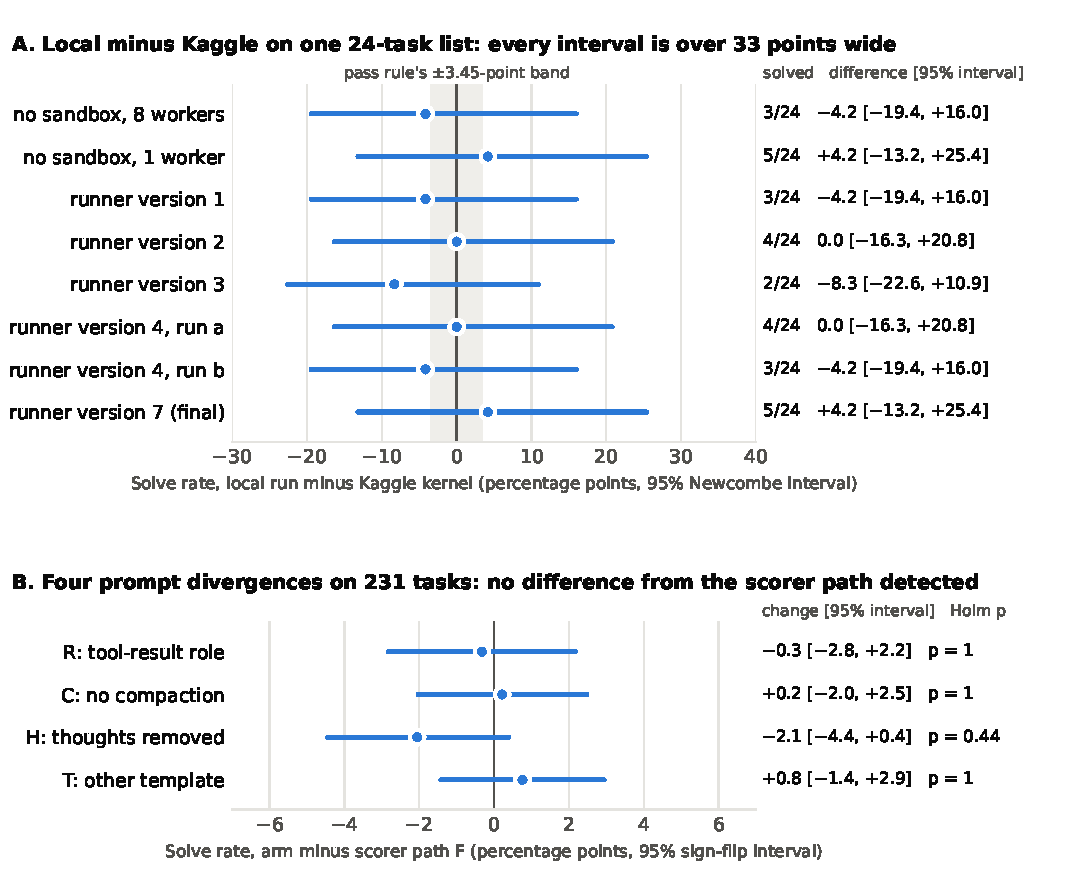
\includegraphics[width=\linewidth]{fig/parity_effects.pdf}
\caption{(A) Solve-rate difference, local minus Kaggle (pooled 8/48), for eight local runs of one 24-task list (95\% Newcombe intervals, runs treated as independent); shaded: the pass rule's \ensuremath{\pm}3.45 points. (B) Change in solve rate against F on 231 tasks: estimates, 95\% intervals and Holm-adjusted p.}\label{fig:parity}
\end{figure}
